\documentclass[a4paper]{article}

\usepackage{geometry}            % for margins
\usepackage{amsthm}              % for theorems, definition, etc.
\usepackage{amssymb}             % for mathcal, mathbb, mathfrak
\usepackage{amsmath}             % for \text
\usepackage{mathrsfs}            % for \mathscr
\usepackage{multicol}            % for \multicols
\usepackage[hidelinks]{hyperref} % for clickable and hidden reference links
\usepackage{float}               % for [H] options in the figure environment
\usepackage{tikz}                % for tikzpicture
\usetikzlibrary{positioning}     % for tikz's relative positioning
\usetikzlibrary{shapes.misc}     % for tikz's relative positioning
\usepackage{makecell}            % for \thread 

\renewcommand\theadfont{\bfseries}

\geometry
{
   left   = 25mm,
   right  = 25mm,
   top    = 25mm,
   bottom = 25mm,
}
\theoremstyle{definition}
\newtheorem{definition}{Definition}

\newcommand{\ra}{\rightarrow}
\newcommand{\ts}{\text{ }}
\newcommand{\mn}{\text{-}}

\begin{document}


\title
{
   Spiking Neural P System Models\\ as Formal Framework Models
}


\author
{
   Ren Tristan A. de la Cruz
}



\maketitle

% ================================================================================================= %

\section{Background}\label{sec-background}

\emph{Membrane computing} is a field of computer science that studies models of computation known as
\emph{P systems}. P systems refer to a family of models of computation that are inspired by 
different biological processes. P systems use biological concepts like cells, cell membranes, 
neurons, tissues, etc. Rules (computing operations) in P systems are inspired by biological 
processes like chemical reactions in cells, ion transport between regions divided by membranes, 
membrane creation, division and dissolution, spiking of neurons, neurogenesis and synaptogenesis, 
etc. P systems are parallel and distributed models of computation. This means a P system can apply 
multiple rules at the same time and these rules maybe applied in different parts or components of
the P
system. 

Most P systems use multisets of object symbols as computing elements. One can think of these symbols
as abstraction of things like molecules or ions. The multisets of symbols are compartmentalized into
regions that are defined by the membranes that enclose them. This is the reason why the field is 
known as `membrane computing'. Regions can be connected to each other. In cell-like P systems, 
membranes inside the cell can be nested. For example, if there are two membranes in a cell, membrane
$0$ and membrane $1$, and membrane $1$ is inside membrane $0$ then the region enclosed by membrane 
$1$ is connected to the region enclosed by membrane $0$ that is outside membrane $1$. In tissue-like 
P systems, membranes represent cells and each cell enclosed one region. Cells (and hence regions) 
can be connected to each other via channels. Tissue P systems form networks of cells. In general, 
the \emph{configuration} of a P system refers to the network of cells or network of membranes where 
each cell or membrane contains a multiset of objects. In some P system models, a cell/membrane has a
state or status that is different from its multiset content. For example, in some cell-like P 
systems, a membrane has a state known as \emph{polarity} or \emph{charge} which can either be 
negative, positive, or neutral.

There are many diverse P system models.  One reason for the diversity of P systems is the diversity 
of the types of rules used by the systems. There are many different types of rules and a P system 
model can use more than one type.  A rule is an operation that transforms the configuration of a P 
system. One can look at a rule as having two components: (1) a set of conditions the configuration 
of a P system has to meet for the rule to be eligible for application, and (2) a set of actions 
(transformations) the rule will apply to the P system's configuration. Different types of rules have
different sets of conditions and different actions since they are inspired by different biological 
processes. For example, one common type of rule is called an \emph{evolution rule}. An 
evolution rule is associated with a region and it consumes a multiset of objects in that region then 
produces another multiset of objects. Evolution rules are inspired by chemical reaction occurring
inside cell membranes. Another example of a rule type is the \emph{communication rule}. In cell-like 
P systems, a communication rule is associated with a membrane and it facilitates a transfer or 
exchange of multisets of objects between the region inside the membrane and the region outside. 
Communication rules are inspired by the ion transfers between regions via ion channels on cell 
membranes. There are also types of rules that transform the network of cells/membranes itself and 
not just the contents of the  cells/membranes. For example, there are rules that can create and 
delete channels between cells. There are also rules that can create and delete membranes/cells. 
These rules are inspired by processes like cell/membrane division, membrane dissolution, neuron 
creation, synapse creation and deletion, etc.

P systems are parallel models so it is possible for the systems to apply different rules at
the same time and they can also apply a rule multiple times. For example, evolution rules are 
inspired by chemical reactions and it is possible for different chemical reactions to occur multiple
times inside cell membranes. P systems have a set of criteria that specifies which combination of
eligible rules are valid. This set of criteria is called the \emph{derivation mode}. Aside from the
types of rules used by P systems, different P systems can also use different derivation modes.
Derivation modes can describe the type of parallelism the P system is working on. For example, the
derivation mode known as \emph{maximal parallelism} only allows combinations of eligible rule 
instances that are \emph{maximal}. In a \emph{maximal} combination of rule instances, one can not
add any additional instance of eligible rules. The maximal combination of rules will consume 
enough  symbols such that the remaining multiset of symbols does not allow any more rules to be 
applied. In a P system working in maximally parallel mode, any combinations of eligibles rules that 
are not maximal are not used. Another common derivation mode is the \emph{minimally parallel} mode. 
In P systems working in minimally parallel mode, cells/membranes with eligible rules can still apply
rules in parallel but each cell/membrane can only apply at most single instance of an eligible rule. 
Derivation modes can also describe rule priorities. For example, in a P system with two types of 
rules, type $A$ and type $B$, one can specify in the model that if any type $A$ rule in a membrane 
is eligible then no (eligible) type $B$ rules can be applied. In the situation where there is an 
eligible type $A$ rule in a membrane, any rule combination that includes an eligible type $B$ rule 
in the same membrane is not valid.

When one combines the different types of rules and the different derivation modes, one can produce
a significant number of diverse P system models. In order to help make sense of the different P 
system models, a \emph{formal framework} was introduced in 2007 by Freund et al. The idea behind the 
formal framework (for P systems) is to have a set of general concepts and constructs that can be 
used when analysing most, if not all, types of P systems. The first version of the formal framework
can be found in \cite{freund-2007-ff-1} and it is a framework for static tissue-like P system.

A system in the formal framework is called a \emph{network of cells}. Similar to most P systems, the 
configuration of a network of cells is defined by the multiset contents of the cells of the system.
The framework has a single type of rule called an \emph{interaction rule}. An \emph{interaction 
rule} is a rule type that generalizes most rule types used by cell-like and tissue-like P systems. 
Most variants of communication rules and evolution rules are special cases of the more general 
interaction rule. Different types of P system rules can have different forms but can also have
different syntax. By formulating P systems as network of cells and using the interaction rule form,
P system rules are written as interaction rules which means they are written to have the same
general form and a common syntax. The interaction rule form makes comparing rules of different P 
systems easier. For example, two rule types from two different P systems may superficially appear 
different, due to different syntax,  but when they are written as interaction rules it appears that 
their eligibility criteria and their actions are actually very similar. In the formal framework, the 
effect of an interaction rule when applied to a configuration is formally defined. This is not 
necessarily the case for other P systems and their rules. In some P system models, the effect of a 
rule on the configuration is described in a less formal manner (describe in plain English) which is 
prone to different interpretations. If one is to write a rule type from one P system model as an
interaction rule, one has to formally define the meaning of the rule. The framework helps one 
clarify the meaning of the rule.

Aside from a general form of a rule, the framework in \cite{freund-2007-ff-1} also lists common
derivation modes used by most P systems. The meaning of those different derivation modes are 
formally defined. In some P systems, derivation modes are less formally defined which again can lead 
to multiple conflicting interpretations. The framework lists other possible derivation modes that
are rarely or not yet used by existing P system models which means they can be used to formulate new
P system models.
 
The formal framework from \cite{freund-2007-ff-1} is limited to static P system. An interaction rule
from \cite{freund-2007-ff-1} can not directly represent a P system rule that changes the structure
of the network of cells, a rule that can create or delete cells or the connections between cells. 
The second version of the formal framework \cite{freund-2013-ff-2} has a much more general form of 
an interaction rule. The interaction rule from \cite{freund-2013-ff-2} can be used to write rules 
that change the structure of the network of cells. The rule form is much more complicated than the 
form of the interaction rules in \cite{freund-2007-ff-1}.

A third version of the formal framework can be found in \cite{verlan-2020-ff-3}. This version is 
an extension of the first version. The main differences between the first and the third version are:
(1) the interaction rule in the third version allows multiset pattern checking and (2) the third
version framework introduces the input and output constructs. In the first version of the framework, 
the criteria for eligibility of interaction rules are combinations of the presence of certain 
multisets in specified regions and the absence of certain multisets in specified regions. In the
third version, the criteria for eligibility of an interaction rule rely on \emph{control languages} 
(the pattern). For example, if certain multisets in specified regions are in the control languages 
of those regions (the multisets `fits the pattern' for those regions), then the rule is eligible. 
Control languages and the input and output constructs are needed to represent P systems known as 
\emph{spiking neural P systems} (SNP systems). SNP systems use a type of rule that checks for 
patterns. Such rules need the concept of a control language in order for them to be represented in 
the framework. SNP systems are also usually used as transducers so it makes sense for the new 
framework to have input and output constructs.

The formal frameworks can be used to understand the functioning of P system variants. This is done
by translating concepts from a P system model to concepts in the framework. Since the concepts in 
the framework are formally defined, the process of translating P system concepts to the language of
the framework forces one to clarify and formalize those concepts that may have been vaguely
described in the P system model. This process is particularly helpful when analysing P system models 
with vague semantics. The process highlights the concepts (e.g. rule semantics) that may have
different interpretations. The formal frameworks can also be used as a common language for comparing
different P systems. By translating different P systems as network of cells in the formal framework, 
the different P systems will have the same general form and will use the same syntax. This makes the
comparison of the models a significantly easier task. The formal frameworks can also be use to
extend P system models with new features. Since the constructs in the formal framework can be seen
as generalized versions of constructs in most P system models (i.e. the formal framework's 
interaction rule is a generalized P system rule), one can add features available in the formal
framework constructs as new features in new P system models. Some of these applications of the 
formal framework can be found in \cite{verlan-2014-ff-2.5}.

%===================================================================================================

This work is focuses on the use of the formal framework concepts and constructs for representing
spiking neural P system models. 

Neural-like P systems known as \textit{spiking neural P systems} (SNP systems) were introduced in    
\cite{ionescu-2006-snp}. They are inspired by the workings of a network of spiking neuron. A 
biological neuron has an electric charge. If the neuron's charge changes and passes a certain 
threshold, the neuron will `spike' and it will send a signal to other connected neurons. This is
where the term `spiking neuron' came from. SNP systems use one type of object called a \emph{spike}. 
An SNP system's neuron stores a multiset of spikes. The multiset of spikes in an SNP system's neuron 
is the analogue of the electric charge in biological neurons. The spiking behavior of an SNP
system's neuron is controlled by a set of rules. The rules look at the multiset of spikes in the
neuron and determine if the neuron should spike or not. These rules are the analogue of the
threshold mechanism in biological neurons. An SNP system is a network of such neurons. The neurons 
are connected to each other using \textit{synapses}. We  will refer to this model (from 
\cite{ionescu-2006-snp}) as the \textit{classic} or \textit{standard} SNP system since there are 
already a lot of SNP system variants that have been introduced.                                  
                                                                                                     
The standard SNP system is based on an simplified and highly abstracted mechanisms of a spiking      
neuron. There are many features and mechanism in the biological neural system that are good sources  
of inspiration for the creation of new SNP system variants. Similar to the standard SNP systems,     
other SNP system variants take some features or mechanisms from the biological neural system,        
abstract and simplify them, and then incorporate the simplified features/mechanisms in the models.   
Some examples of these variants are: SNP systems with weighted synapses
\cite{wang-2010-weights,pan-2012-weighted-synapses}, SNP systems with inhibitory rules 
\cite{peng-2019-inhibitory-rules}, SNP systems with astrocytes 
\cite{paun-2007-astrocyte-like,pan-2012-astrocytes}, SNP systems with 
neuron division, budding, and dissolution
\cite{wang-2011-neuron-division,pan-2011-division-budding,zhao-2016-division-dissolution}, 
SNP systems with dynamics synapses 
\cite{cabarle-2015-structural-plasticity,cabarle-2017-scheduled-synapses},
SNP systems with polarizations \cite{wu-2018-polarizations}, and SNP systems with thresholds         
\cite{zeng-2014-thresholds}.                                                                         

Other SNP system models can be almost exactly similar to an existing SNP system model but only 
having different derivations modes. For example, the standard SNP system works in minimally parallel
mode while the following SNP models are almost exactly similar to standard SNP system except for 
working on a different derivation modes:  SNP systems in \cite{ionescu-2007-exhaustive} use 
exhaustive mode, SNP systems in \cite{cavaliere-2009-asynchronous} use asynchronous mode, SNP 
systems in \cite{ibarra-2009-min-max-sequential} use sequential mode, SNP systems in 
\cite{song-2013-local-sync} use asynchronous mode with local synchronization, and SNP systems in                                 
\cite{zhang-2014-general-rule-use,jiang-2019-improved-usnp-general-rule-use} use a generalized       
derivation mode.

SNP system variants are different from each other because they have different features (i.e. 
different types of rules), different derivation modes, or a combination of both. Aside from being 
inspired by neural system features and mechanisms, some SNP system variants also adopt features from 
other (non-SNP) P systems or get inspiration from other physical or biological phenomena. Other 
SNP system variants can be found in                                                                                      
\cite{chen-2008-snp-e,alhazov-2006-esnp,chen-2007-axon-p,pan-2009-anti-spikes,song-2014-rules-on-synapses,metta-2014-cooperating-rules,wu-2016-cell-like,song-2016-request-rules,pan-2017-communication-on-request,song-2018-colored-spikes}  

As mentioned above, the third version of formal framework \cite{verlan-2020-ff-3} is an extension of 
the first version and the modifications/extensions are made in order to represent SNP systems. In 
\cite{verlan-2020-ff-3}, after defining and describing the constructs of the framework, the authors 
translated the standard SNP system model (with rules without delay) as formal framework's network of 
cells. Standards SNP system's rules are translated as interaction rules. The authors also translated
 rules of other SNP systems variants
\cite{chen-2008-snp-e,pan-2012-weighted-synapses,alhazov-2006-esnp,peng-2017-multiple-channels,pan-2012-astrocytes} 
as interaction rules.  

ADD RESULTS AND SUMMARY HERE

% ================================================================================================= %

\section{Preliminaries}\label{sec-preliminaries}

This section present preliminary concepts used by SNP system models and the formal framework.

The following sets will be commonly used throughout the document: $\mathbb{N} = \{0,1,2,3,...\}$,
$\mathbb{N}_{\infty} = \mathbb{N} \cup \{\infty\}$, $[1..n] = \{1,...,n\}$, 
$2^{[1..n]}=\mathcal{P}([1..n])$ (power set of $[1..n]$).

Let $V$ be a set of symbols called an \emph{alphabet}. A \emph{string} or \emph{word} over $V$ is
a sequence of symbols from $V$. The \emph{empty string} $\epsilon$ is a string without symbols, an 
empty sequence. A \emph{string language} over $V$ is a set of strings over $V$. The set of all 
strings over $V$ is denoted by $V^*$.

A \emph{multiset} over $V$ is a function of the form $m: V \ra \mathbb{N}_{\infty}$ while a
\emph{finite multiset} over $V$ is a function of the form $m: V \ra \mathbb{N}$. If $m$ is a
multiset over $V$ and $a \in V$, $m(a)$ denotes the number of occurrences of symbol $a$ in multiset
$m$. If $V=\{v_1,...,v_k\}$ and $m$ is a finite multiset over $V$, $m$ can be represented by the
string ${v_1}^{m(v_1)}\cdots {v_k}^{m(v_k)}$. The size of a multiset $m$ over $V$ is
$|m| = \sum_{v\in V}m(v)$. An \emph{empty multiset} $\emptyset$ is any multiset of size $0$. An
\emph{infinite multiset} is a multiset with an infinite size. i.e. Multiset $m$ over $V$ is infinite
if for some $v\in V$, $m(v) = \infty$. A \emph{multiset language} over $V$ is a set of multisets 
over $V$. The set of all multisets over $V$ is denoted by $V^{\circ}$.

Let $V=\{v_1,...,v_k\}$, $m$ be the multiset ${v_1}^{m(v_1)}\cdots{v_k}^{m(v_k)}$ and $n$ be the  
multiset ${v_1}^{n(v_1)}\cdots{v_k}^{n(v_k)}$. $m \subseteq n$ if and only if for all $v \in V$ 
$m(v) \leq n(v)$. $m+n$ is the multiset ${v_1}^{m(v_1)+n(v_1)}\cdots {v_k}^{m(v_k)+n(v_k)}$. If 
$m \subseteq n$, $n-m$ is the multiset ${v_1}^{n(v_1)-m(v_1)}\cdots {v_k}^{n(v_k)-m(v_k)}$

The set of all $n$-vectors whose components are finite multisets over $V$ is denoted by
${V^{\circ}}^{n}$. Let $X=(x_1,...,x_n), Y=(y_1,...,y_n) \in {V^{\circ}}^n$. $X \subseteq Y$ if and
only if $x_i \subseteq y_i$ for $1 \leq i \leq n$. $X+Y = (x_1 + y_1,...,x_n + y_n)$. If 
$X \subseteq Y$, $Y-X = (y_1-x_1,...,y_n-x_n)$. An $n$-vector whose components are all empty 
multisets is denoted by $\emptyset_n$. i.e. $\emptyset_n = (\emptyset,...,\emptyset)$. i

A \emph{family of languages} is a set of languages. It can either be a family of string languages or 
a family of multiset languages. The notations $\mathscr{F}$ and $\mathscr{F}^{\circ}$ will be used
for a family of string languages and a family of multiset languages, respectively. The notation
$\mathscr{F}(V)$ will be used for a family of string languages over alphabet $V$ while 
$\mathscr{F}^{\circ}(V)$ will be used for a family of multiset languages over alphabet $V$. For
example, $REG$ is the set regular string languages, $REG(V)$ is the set of regular string 
languages over $V$, $REG^{\circ}$ is the set of regular multiset languages, and $REG^{\circ}(V)$ 
is the set of regular multiset languages over $V$.

A \emph{regular expression over alphabet} $V$ is a string over the alphabet $V_{reg} = V \cup 
\{*,(,),\cup,|\}$ with a particular form. The regular expression defines a string language over $V$.
Any language definable using a regular expression is called a \emph{regular language}. The set of 
all regular expressions over $V$ can be defined recursively. The empty string $\epsilon$ is a 
regular expression and it defines the empty language $\emptyset$. If $v \in V$, then $v$ is a
regular expression that defines the language $\{v\}$. Let $E$ be a regular expression, $L(E)$ 
denotes the languages defined by regular expression $E$. If $E_1$ and $E_2$ are regular expressions
over $V$, then $E_1 \cup E_2$ is a regular expression over $V$ that defines the language
$L(E_1) \cup L(E_2)$, $E_1 | E_2$ or simply $E_1 E_2$ is a regular expression that defines the
language $\{w_1 w_2\ts|\ts w_1\in L(E_1),\ts w_2\in L(E_2)\}$, $(E_1)$ is a regular expression that
similar to $E_1$ also defines the language $L(E_1)$, and ${E_1}*$, written as ${E_1}^*$, is a 
regular expression that defines the language $\{w^n\ts |\ts w\in L(E_1),\ts n\in \mathbb{N}\}$. An 
\emph{extended regular expression} over $V$ is as string over $V_{exreg} = V \cup \{*,(,),\cup,|,',
\cap\}$. The set of extended regular expressions over $V$ is defined in a similar manner to the
recursive definition of the set of regular expression over $V$ but with the following additional
rules. If $E_1$ and $E_2$ are extended regular expressions over $V$, then $E_1 \cap E_2$ is an
extended regular expression that defines the language $L(E_1) \cap \L(E_2)$ and $E_1'$ is an
extended regular expression that defines the language $V^*\backslash L(E_1)$, the complement of the
language $L(E_1)$. Extended regular expressions also define regular languages. A language defined by
an extended regular expression can also be defined by a non-extended regular expression.  The 
complement symbol/operator ($'$) and the intersection symbol/operator ($\cap$) are added in order to 
make expressions that define languages more succinct. A regular language defined by some regular
expression $E_1$ can possibly be defined by a shorter extended regular expression $E_2$. For the
rest of the document, the term `regular expression' will be used for both extended and non-extended
regular expressions.

Since multisets can be represented as strings, regular expressions can also be used to define 
\emph{regular multiset languages}. A regular multiset language over $V$ can be defined by a regular
expression over $V$ of a particular form. Given the alphabet $V = \{v_1,...,v_n\}$, a regular 
expression that defines a multiset language has the form $E_1|E_2|E_3|\cdots|E_n$ where, for $1 \leq
i \leq n$, $E_i$ is a regular expression over $\{v_i\}$. A regular expression $E=E_1|E_2|\cdots|E_n$
defines the multiset language $\{m\ts|\ts \text{string representation of $m$ is in $L(E)$}\}$. 
$L^{\circ}(E)$ denotes the multiset language defined by the regular expression $E$.

% ================================================================================================= %

\section{Formal Framework for Spiking Neural P Systems}\label{sec-ff}

This section presents the constructs from the third version of the formal framework 
\cite{verlan-2020-ff-3} and some constructs from the first version of the framework 
\cite{freund-2007-ff-1} that were no longer presented in \cite{verlan-2020-ff-3}.

% ================================================================================================= %

\definition{}\label{def-conf} \textbf{[Configuration]} An $n$-degree \emph{configuration} 
$C = (u_1,...,u_n)$ over alphabet $V$ is an $n$-vector of multisets over $V$. A configuration $C$ is 
called a \emph{finite configuration} if all the components are finite multisets. A configuration is 
referred to as a \emph{full configuration} to specify that the configuration can contain infinite 
multisets.

In the context of a \emph{network of cells} (defined in full in Definition \ref{def-nc}), an
$n$-degree configuration $C = (u_1,...,u_n)$ represents $n$ cells and the component $u_i$ is the
multiset of objects contained in \emph{cell $i$}.

% ================================================================================================= %

\definition{}\label{def-rule} \textbf{[Interaction Rule]} An $n$-degree \emph{interaction rule} over
alphabet $V$ is the construct $(X \ra Y; K)$ where $X=(x_1,...,x_n)$ and $Y=(y_1,...,y_n)$ 
are $n$-vectors of multisets over $V$ and $K = (k_1,...,k_n)$ is an $n$-vector of multiset
languages.

A interaction rule acts on a configuration by consuming multisets of objects from the configuration
and also producing multisets of objects in the configuration given that a certain set of conditions
is met. The $n$-vector $X$ contains the multisets $x_1,...,x_n$ that the rule will `consume' while
the $n$-vector $Y$ contains the multisets $y_1,...,y_n$ that the rule will produce. The $n$-vector 
$K$ contains multiset languages $k_1,...,k_n$, called \emph{control languages}, that are used to 
check a rule's \emph{eligibility} (in Definition \ref{def-elig}) with respect to some configuration.

A rule can also be written as:
$$(1,x_1)\cdots(n,x_n)\ra (1,y_1)\cdots(n,y_n)\ts;\ts (1,k_1)\cdots(n,k_n)$$

where any component $(i,x_i)$, or $(i,y_i)$, can be omitted if $x_i = \emptyset$, or 
$y_i = \emptyset$, and any component $(i,k_i)$ can be omitted if $k_i = V^{\circ}$. To have a more
compact notation, components $(i,x_i)$, $(i,y_i)$, $(i,k_i)$ can be written as ${[x_i]}_i$,
${[y_i]}_i$, and ${[k_i]}_i$, respectively. Additionally, the control language components of the 
rule can be written first followed by a slash instead of a semicolon then the $X$ and $Y$ 
components. The rule can be written as:

$${[k_1]}_1\cdots{[k_n]}_n\ts / \ts {[x_1]}_1\cdots {[x_n]}_n \ra {[y_1]}_1\cdots{[y_n]}_n$$

The rule syntax above will be used since it is closer to the syntax of most rules in different SNP 
system models. It is organized in such a way that all the components of a rule on the left side
of the arrow, ${[k_1]}_1 ... {[k_n]}_n/{[x_1]}_1...{[x_n]}_n$, are the criteria for rule eligibility
while all the components on the right side of the slash, 
${[x_1]}_1\cdots {[x_n]}_n \ra {[y_1]}_1\cdots{[y_n]}_n$, represent the actions that will be 
performed if the rule is applied. The ${[x_1]}_1...{[x_n]}_n$ components specify both eligibility
criteria and actions of the rule.

% ================================================================================================= %

\definition{}\label{def-elig} \textbf{[Rule Eligibility]} Let $C = (u_1,...,u_n)$ be an $n$-degree
configuration over $V$ and $r = ((x_1,...,x_n) \ra (y_1,...,y_n);$ $(k_1,...,k_n))$ be an $n$-degree
rule over $V$, rule $r$ is \emph{eligible} with respect to configuration $C$ if the following 
conditions hold: (1) for all $x_i$, $x_i \subseteq u_i$ and (2) for all $u_i$, $u_i \in k_i$.

Since the rule consumes the multisets $x_1,...,x_n$ from configuration $C$ ($x_i$ is consumed from
cell $i$), the first condition $x_i \subseteq u_i$ states that (for all cells) content $u_i$ of cell
$i$ should have enough objects in order for the rule to consume the multiset $x_i$ of objects from
the cell. The second condition simply checks if the content $u_i$ of cell $i$ is in the control
language $k_i$ associated with the cell.

% ================================================================================================= %

\definition{}\label{def-appc} \textbf{[Applicability of a Multiset of Rules]} Let $R'$ be a multiset 
of $n$-degree rules over $V$ and $C = (u_1,...,u_n)$ be an $n$-degree configuration over $V$, $R'$ 
is \emph{applicable} to configuration $C$ if the following conditions hold: (1) each rule 
$(X_j \ra Y_j;K_j) \in R'$ is eligible with respect to configuration $C$ and (2) 
$$X = \Bigg(\sum_{\substack{(X_j \ra Y_j; K_j) \in R'}} X_j\Bigg)\subseteq C.$$

The applicability of a multiset of rules is simply an extension of the concept of rule eligibility
to a multiset of rules. For a multiset $R'$ of rules to be applicable, all rules in $R'$ should
be eligible (condition 1) and there should be enough objects in the configuration's cells to be 
consumed by all rules in $R'$ (condition 2). Vector $X$ represents total multisets of objects that 
will be consumed per cell by all the rules in $R'$.

% ================================================================================================= %

\definition{}\label{def-appl} \textbf{[Application of a Multiset of Rules]} If $R'$ is multiset of 
rules applicable to configuration $C = (u_1,...,u_n)$, \emph{applying} $R'$ to configuration $C$ 
means producing a new configuration $C'$ which is defined as: 
$$C' = Apply(R',C) =  C - \Bigg(\sum_{\substack{(X_j \ra Y_j; K_j) \in R'}} X_j\Bigg) +
\Bigg(\sum_{\substack{(X_j \ra Y_j; K_j) \in R'}} Y_j\Bigg).$$

The \emph{application function} $Apply(R',C)$, as defined above, takes an applicable multiset of 
rules $R'$ and configuration $C$ and outputs a new configuration $C'$. Configuration $C'$ is the 
result of removing all multisets of objects consumed by all rules in $R'$ from configuration $C$ and 
then adding all multisets of objects produced by all rules in $R'$ to configuration $C$.

% ================================================================================================= %

\definition{}\label{def-nc} \textbf{[Network of Cells]} A $\mathscr{F}$-controlled \emph{network of 
cells} of degree $n$ is the construct $$\Pi = (n, V, W, c_{in}, c_{out}, R)$$ where

\begin{multicols}{2}
\begin{itemize}
\item $n$ is the number of cells; 
\item $V$ is a finite alphabet;
\item $W = (w_1,...,w_n)$ is the \emph{initial configuration} where $w_i \in V^{\circ}$ is the
      multiset associated with cell $i$.
\item $c_{in} \subseteq [1..n]$ is the set of \emph{input cells}.
\item $c_{out} \subseteq [1..n]$ is the set of \emph{output cells}.
\item $R$ is the set of interactive rules. 
\end{itemize}
\end{multicols}

The primary components of a network of cell (system) are its initial configuration $W$ and its set 
of interactive rules $R$. The first two components of a network of cells specify the degree and the 
alphabet used by the system. This means that the configuration and the rules of the system are of 
degree $n$ and over alphabet $V$. $c_{in}$ is the set of cell \emph{ids or labels} that specifies 
the set of input cells while $c_{out}$ is the set of cell ids or labels that specifies the set of 
output cells.

If system $\Pi$ is $\mathscr{F}$-controlled, it means all control languages used by the rules of
$\Pi$ belong to the family of languages $\mathscr{F}$. More specifically, the control languages used
by the system $\Pi$ belong to the family $\mathscr{F}^{\circ}(V)$ of multiset languages over $V$.

During computation, a network of cells changes its configuration. If a system $\Pi$ has the
configuration $C$, $Applicable(\Pi,C)$ is the set of all multiset of rules (rules from $R$ of $\Pi$) 
applicable to $\Pi$'s current configuration $C$.

% ================================================================================================= %

\definition{}\label{[def-nc2]}\textbf{[Network of Cells with Environment]} An 
$\mathscr{F}$-controlled \emph{network of cells with environment} of degree $n$ is the construct:

$$\Pi_{inf} = (\Pi,Inf) = ((n,V,W,c_{in},c_{out},R), Inf)$$
\begin{itemize}
\item The first component $\Pi_{inf}$ is as defined in Definition \ref{def-nc}.
\item $Inf = (inf_1,...,inf_n)$ where $inf_i \subseteq V$ is a \emph{set of symbols occurring 
infinitely often in cell i}.
\end{itemize}

A network of cells with environment is an extension of the network of cells concept. A network of
cells with environment allows infinite multisets. $Inf=(inf_1,...,inf_n)$ is an $n$-vector of sets 
of symbols (symbols from $V$). $inf_i$ is a set of symbols associated with cell $i$. All symbols in 
$inf_i$ occurs infinitely often in cell $i$. If $inf_i$ is not empty, then cell $i$ contains an
infinite multiset. 

% ================================================================================================= %

\definition{}\label{def-derv} \textbf{[Derivation Mode]} A \emph{derivation mode} $\delta$ is a
restriction of the set of applicable rules. For network of cells $\Pi$ and configuration $C$, 
$Applicable(\Pi, C, \delta) \subseteq Applicable(\Pi, C)$ denotes the set of multisets of
rules in $\Pi$ applicable to configuration $C$ according to derivation mode $\delta$. 

\emph{Maximal parallelism} or \emph{maximally parallel} derivation mode is one of the most commonly
used derivation modes. A maximally parallel network of cells only uses applicable multisets of rules
whose size is already maximal. i.e. One can not add additional instances of eligble rules to a
maximal multiset of rules without making the (new) multiset of rules non-applicable (there are not 
enough objects for the new multiset of rules to consume). Another common derivation mode is 
\emph{minimal parallelism} or \emph{minimally parallel} derivation mode. In this mode, rules of the 
system $\Pi$ are grouped into non-intersecting partitions. Only applicable multisets of rules that 
have at most one instance of rule for each of the partition are used in this mode. Maximal 
parallelism, minimal parallelism and other derivations modes are listed in detail in Appendix 
\ref{app-derivation}.

% ================================================================================================= %

\definition{}\label{def-nc3}\textbf{[Network of Cells Working in $\delta$ Derivation Mode]} An
$\mathscr{F}$-controlled $n$-degree \emph{network of cells working in $\delta$ derivation mode} is 
the construct: $$\Pi' = (\Pi,\delta) = ((n,V,W,c_{in},c_{out},R), \delta)$$
\begin{itemize}
\item The first component $\Pi$ is as defined in Definition \ref{def-nc}.
\item $\delta$ is the derivation mode used.
\end{itemize}

$NC(n,V,\mathscr{F},\delta)$ is the set of $n$-degree $\mathscr{F}$-controlled network of cells 
using alphabet $V$ and working in $\delta$ derivation mode.

% ================================================================================================= %

\definition{}\label{def-comp1}\textbf{[Computation of a Network of Cells]} A \emph{computation} of
a network of cell $\Pi' = ((n,V,W,c_{in},c_{out},R),\delta)$ is sequence a $C_0,C_1,C_2,...$ of
configurations of $\Pi$ with the following properties:
\begin{itemize}
\item $C_0 = W$
\item $C_{i+1} = Apply(R',C_i)$ where $R' \in Applicable(\Pi,C_i,\delta)$.
\end{itemize}

% ================================================================================================= %

\definition{}\label{def-input} \textbf{[Input Function]} An \emph{input function} for a system 
$\Pi'=((n,v,W,c_{in},c_{out},R),\delta)$  is a function of the form $Input(\Pi'): \mathbb{N} \ra 
{V^{\circ}}^{n}$ and fulfills that condition that for all $i \notin c_{in}$ the $i$-th component of 
resulting input vector from ${V^{\circ}}^n$ is an empty multiset.

The input function takes a number representing a time step in the computation, say $t$, as input 
and produces an $n$-vector, say $I$, of multisets over $V$. i.e. $Input(\Pi')(t) = I$. Only the
$j$-th components, where $j \in c_{in}$, are allowed to be non-empty multisets since $c_{in}$
specifies the input cells that are allowed to take non-empty input multisets.

% ================================================================================================= %

\definition{}\label{def-comp2}\textbf{[Computation with Input of a Network of Cells]} A 
\emph{computation with input} of a network of cell $\Pi' = ((n,V,W,c_{in},c_{out},R),\delta)$ is a 
sequence a $C_0,C_1,C_2,...$ of configurations of $\Pi$ with the following properties:
\begin{itemize}
\item $C_0 = W + Input(\Pi')(0)$
\item $C_{i+1} = Apply(R',C_i) + Input(\Pi')(i+1)$ where $R' \in Applicable(\Pi, C_i, \delta)$.
\end{itemize}

If the context is clear, a computation with input will simply be called a computation.

%===================================================================================================

\definition{}\label{def-output} \textbf{[Output Function]} An \emph{output function} 
$Output(\Pi',C)$ for a system $\Pi' = ((n,V,W,c_{in},$ $c_{out},R),\delta)$ and a computation 
$C=C_0,C_1,C_2,...$ of system $\Pi'$ is a function that takes a number representing a time step
as input and produces an output derived from the finite computation $C_0,...,C_t$.

The output of a system $\Pi$ depends on how the system is being used. For example, the system $\Pi$
can be used to compute a number and this number is represented as a multiset in a particular cell in
$\Pi$. For this case, the output function simply returns the multiset of the specified cell for a 
given time $t$ or it can return the number itself represented by the multiset. System $\Pi$ can also 
be used to generate a string where the $i$-th character of the string is represented by the multiset 
in a particular cell in the $i$-th configuration $C_i$ of the computation. In this case, the output 
function for system $\Pi$ and computation $C$ returns the said string.

% ================================================================================================= %

\definition{}\label{def-halt}\textbf{[Halting Condition]} A \emph{halting condition} is a condition
placed on a finite computation $C$ of a system $\Pi'$ that determines if the computation is a 
\emph{halting computation} and that system $\Pi'$ halts after computation $C$.

The most commonly used halting condition is the \emph{total halting} condtion. Total halting states
that a computation $C = C_0,...,C_t$ of a system $\Pi'=(\Pi,\delta)$ is a halting computation if 
$Applicable(\Pi,C_t,\delta) = \emptyset$. i.e. There are no applicable multiset of rules (in 
$\delta$ derivation mode) for configuration $C_t$. Commong halting conditions are listed in detail
in Appendix \ref{app-halt}.

%===================================================================================================

\section{Spiking Neural P System Models as Formal Framework Network of Cells}\label{sec-snp}

This section looks at different SNP system models as networks of cells. Concepts and constructs from
the different SNP system models are translate to concepts and construct in the formal framework.  

\subsection{Spiking Neural P System}

\definition{}\label{def-snp} \textbf{[Spiking Neural P System]} A \emph{spiking neural P system
(SNP system)} \cite{ionescu-2006-snp} of degree $n$ is the construct:

$$\Pi = (O, \sigma_1,...,\sigma_n,syn,i_o)$$

\begin{itemize}
\item $O = \{a\}$ is the singleton alphabet of the system. Symbol $a$ is called a \emph{spike}.
\item $\sigma_1,...,\sigma_n$ are neurons of the form
      \begin{itemize}
      \item $\sigma_i = (n_i, R_i)$ for $1 \leq i \leq n$. 
      \item $n_i \in \mathbb{N}$ is initial number of spikes in neuron $i$. 
      \item $R_i$ is a finite set of rules of the following two forms:
            \begin{itemize}
            \item \emph{Spiking Rule:} $E/a^c \ra a;d$ where $E$ is regular expression over $O$, 
                  $d \in \mathbb{N}$,$c \in \mathbb{N}\backslash \{0\}$.
            \item \emph{Forgetting Rule:} $a^s \ra \lambda$ where $s \in \mathbb{N}\backslash\{0\}$\
                  and $\{a^s\} \cap L^{\circ}(E) = \emptyset$ for all $E$ that are regular 
                  expressions of a spiking rules in the same neuron.
            \end{itemize}
      \end{itemize}
\item $syn \subseteq [1..n] \times [1..n]$ is the set of \emph {synapses} where $(i,i) \notin syn$ 
      for all $i \in [1..n]$.
\item $i_o \in [1..n]$ specifies the \emph{input neuron} in accepting mode or the \emph{output
      neuron} in generating mode.
\end{itemize}

Standard SNP systems of degree $n$, as networks of cells, belong to the family 
$NC(n,O,REG^{\circ}(O), min)$. They use the alphabet is $O =\{a\}$. All control languages used by 
the rules are from the family $REG^{\circ}(O)$ which is the family of regular multiset languages 
over $O$. The systems work under minimal parallelism ($\delta = min$) where rules in the system are
partitioned in such a way that each neuron has its own set of rules and only combinations of rules 
where at most $1$ rule is used per neuron are allowed.

A spiking rule $E/a^c \ra a;d$ in neuron $i$ is eligible if the multiset $m_i = a^{n_i}$ in the
neuron $i$ is in the multiset languages $L^{\circ}(E)$ and the number of spikes $n_i$ is at least
$c$. If the rule is applied, at step $t$, $c$ spikes are consumed changing the spike count of the
neuron to $n_i-c$, the neuron `closes' for $d$ time steps from time step $t$ to time step $t+d-1$, 
then the neuron will send a spike at time $t+d$ to all other neurons adjacent to neuron $i$ i.e.
Neuron $i$ will send a spike to all neuron $j$ such that $(i,j) \in syn$. The $d$ compnent of the
rule is called the \emph{delay} since it delays the rule from sending out spikes. When a neuron is 
closed, it can neither receive spikes nor activate a rule. A forgetting rule $a^s \ra \lambda$ in 
neuron $i$ is eligible if the multiset $m_i$ in the neuron is $a^s$. When the forgetting rule is 
applied, all $s$ spikes in the neuron are consumed changing the spike count in the neuron to $0$.

An $n$-degree SNP system's configuration is the construct $(m_1/t_1,...,m_n/t_n)$ where $m_i$ is
the multiset of spikes in neuron $i$ while $t_i \in \mathbb{N}$ is the \emph{state} of neuron $i$.
Neuron $i$ is in an \emph{open state} if $t_i = 0$ otherwise it is in a \emph{closed state} if
$t_i > 0$. $t_i$ also represents the time delay before the active rule in neuron $i$ sends a spike
out.

To simplify the formal framework, the delay component of the spiking rule is not incorporated to the
framework's interaction rule. This is not very restrictive, in terms of computability, since it was
shown in \cite{ibarra-2007-snp-normal} that the SNP system model that only has spiking rules without 
delay (i.e. all spiking rules have $d = 0$, simply written as $E/a^c \ra a$) is still 
turing-complete. This also means that the configuration of the system is simply the $n$-vector
$(m_1,...,m_n)$ of the multisets of spikes of the neurons. 

An \textbf{SNP system's spiking rule (without delay)} $\mathbf{E/a^c \ra a}$ in neuron $i$ can be 
written as the formal framework interaction rule: 

$${[L^{\circ}(E)]}_i/ {[a^c]}_i \ra {[a]}_{j_1} \cdots [a]_{j_k}$$

where neurons $j_1,...,j_k$ are neurons adjacent to neuron $i$. i.e. $(i,j) \in syn$ for $j \in \{
j_1,...,j_k\}$, as shown in Figure \ref{fig-snp}.

\begin{figure}[H]
\begin{center}                                                                                           
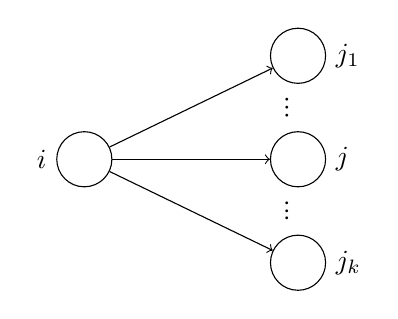
\begin{tikzpicture}
[
scale=1.0,
neuron-a/.style={circle,draw,minimum size = 07mm},
text-a/.style={black},
]
\node (n1) [neuron-a] at (0,0) {$ $};
\node (l1) [text-a,   left  = 00mm of n1]              {$i$};
\node (n2) [neuron-a, right = 20mm of n1]              {$ $};
\node (l2) [text-a,   right = 00mm of n2]              {$j$};
\node (d1) [text-a,   above = 03mm of n2, rotate =90]  {$...$};
\node (n3) [neuron-a, above = 06mm of n2]              {$ $};
\node (l3) [text-a,   right = 00mm of n3]              {$j_1$};
\node (d2) [text-a,   below = 03mm of n2, rotate =270] {$...$};
\node (n4) [neuron-a, below = 06mm of n2]              {$ $};
\node (l4) [text-a,   right = 00mm of n4]              {$j_k$};
\draw [->] (n1) -- (n2) node[midway, below] {$ $};
\draw [->] (n1) -- (n3) node[midway, below] {$ $};
\draw [->] (n1) -- (n4) node[midway, below] {$ $};
\end{tikzpicture}                                                                                        
\end{center}                                                                                             
\caption{Neuron $i$ and Adjacent Neurons $j_1,...j_k$}\label{fig-snp}
\end{figure} 

An \textbf{SNP system's forgetting rule} $\mathbf{a^s \ra \lambda}$ in neuron $i$ can be written as 
the interaction rule:

$${[L^{\circ}(E)]}_i\ts/\ts {[a^c]}_i \ra \emptyset_n$$

Originally, SNP systems have been used to accept or generate sets of numbers. An SNP system in 
\emph{accepting mode} is used to accept a set of numbers. Neuron $i_o$ is the specified input 
neuron. The input neuron will receive two spike, one spike at time $t_1$ and another spike at time
$t_2$. The difference $n = t_2-t_1$ between the arrival time of the first spike and second spike
is the input to the system. Number $n$ is accepted by the system if the system halts on the input.
Total halting is the halting condition used by the SNP system model. 

The function below is the input function used by the system $\Pi'$ (network of cells representation
of SNP system $\Pi$):

$$Input(\Pi')(t) = Z^{(t)} = (z_1^{(t)},...,z_{i_o}^{(t)},...,z_n^{(t)}) =
(\emptyset,...,z_i^{(t)},...,\emptyset)$$
\[
z_{i_o}^{(t)} =
\begin{cases} 
a           & ,\ts t \in \{t_1,t_2\} \\
\emptyset   & ,\ts t \notin \{t_1,t_2\}
\end{cases}
\]

An SNP system in \emph{generating mode} is used to generate a set of numbers. Neuron $i_o$ is the
specified output neuron. The number generated by the SNP system is represented by the difference
$n = t_2 - t_1$ between time $t_1$ when neuron $i_o$ first spikes and time $t_2$ when neuron $i_o$
spikes for the second time. The function below is the output function used by network of cells 
$\Pi'$:

\[
Output(\Pi',C)(t) = 
\begin{cases}
n = t_2 - t_1 &, \text{if output neuron spikes at least once in $t$ steps}\\
\infty        &, \text{if output neuron has not spike yet in $t$ steps} 
\end{cases}
\]

$C = C_1, C_2,C_3,...$ is the computation of $\Pi'$. Both $t_1$ and $t_2$ can be determined by 
looking at the different configurations in computation $C$ then the output function can simply 
return $n = t_2 -t_1$. 

The $n$-degree SNP system $\Pi$, as defined in Definition \ref{def-snp} (except all spiking rules 
have delay $d=0$), can be represented by the formal framework's $REG^{\circ}$-controlled network of 
cells:
$$\Pi'= ((n,O,W=(w_1,...,w_n),c_{in}=\emptyset, c_{out}=\{i_o\}, R),\delta=min) 
\text{ where } w_i = a^{n_i} \text{ (in generating mode)}$$ 
$$\Pi'= ((n,O,W=(w_1,...,w_n), c_{in}=\{i_o\}, c_{out}=\emptyset, R),\delta=min) 
\text{ where } w_i = a^{n_i} \text{ (in accepting mode)}$$ 

%===================================================================================================

\subsection{Spiking Rules as Interaction Rules}

This section looks at how different spiking rules from different SNP system variants can be written 
as interaction rules. Different SNP system variants that are very similar to each other when one
looks at them as network of cells. As networks of cells, they all have the same components (i.e. 
same alphabet, same configuration, same input/output functions, same derivation mode, etc). The only 
difference is the form of the interaction rules that they use. The different versions of spiking 
rules used by the different SNP system variants in this section are simply restricted versions of an 
interaction rule, interaction rules with specific forms. This is not always the case since there are
spiking rule variants that can not be written as one interaction rule. The original spiking rule 
with delay is a simple example. We will only deal with non-delayed version of the different spiking 
rule variants in this section.

An SNP system variant in \cite{chen-2008-snp-e} has a spiking rule of the form $E/a^c \ra a^p$. This 
rule called an \emph{extended spiking rule}. The extended spiking rule is a generalization of the 
original spiking rule. In an extended spiking rule, one can specify the number of spikes to be sent
out to adjacent neurons. This is specified by the multiset $a^p$ ($p$ spikes are sent out). If the
spiking rule is in neuron $i$ and there are synapses from neuron $i$ to neurons $j_1,...,j_k$ (see
Figure \ref{fig-snp}), then its corresponding interaction rule is: 
$${[L^{\circ}(E)]}_i\ts/\ts {[a^c]}_i \ra {[a^p]}_{j_1} \cdots {[a^p]}_{j_k}$$


A variant called \emph{SNP systems with weighted synapses} \cite{pan-2012-weighted-synapses} has the
additional feature having positive integer weights on its synapses. A spike sent through a synapse 
with weight $w$ will arrive as $w$ spikes at the target neuron. The spiking rule in this variant 
has the same form as an extended spiking rule, $E/a^c \ra a^p$. If the rule is activated, the neuron
will send out $p$ spikes through its outgoing synapses. The weight of the synapse will be a
multiplier and the $p$ spikes sent through a synapse with weight $w$ will arrive at the target 
neuron as $p\cdot w$ spikes. If a spiking rule $E/a^c \ra a^p$ is in neuron $i$ and neuron $i$ is 
connected to neurons $j_1,...,j_k$ where the weight of synapse $(i,j_q)$ is $w_q$ ($1 \leq q \leq 
k$), see Figure \ref{fig-snp2}, then its corresponding interaction rule is:

$${[L^{\circ}(E)]}_i\ts/\ts {[a^c]}_i \ra {[a^{p \cdot w_{1}}]}_{j_1} \cdots 
{[a^{p\cdot w_{q}}]}_{j_q} \cdots {[a^{p\cdot w_{k}}]}_{j_k}$$

\begin{figure}[H]
\begin{center}                                                                                           
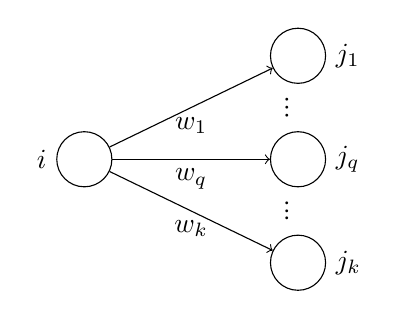
\begin{tikzpicture}
[
scale=1.0,
neuron-a/.style={circle,draw,minimum size = 07mm},
text-a/.style={black},
]
\node (n1) [neuron-a] at (0,0) {$ $};
\node (l1) [text-a,   left  = 00mm of n1]              {$i$};
\node (n2) [neuron-a, right = 20mm of n1]              {$ $};
\node (l2) [text-a,   right = 00mm of n2]              {$j_q$};
\node (d1) [text-a,   above = 03mm of n2, rotate =90]  {$...$};
\node (n3) [neuron-a, above = 06mm of n2]              {$ $};
\node (l3) [text-a,   right = 00mm of n3]              {$j_1$};
\node (d2) [text-a,   below = 03mm of n2, rotate =270] {$...$};
\node (n4) [neuron-a, below = 06mm of n2]              {$ $};
\node (l4) [text-a,   right = 00mm of n4]              {$j_k$};
\draw [->] (n1) -- (n2) node[midway, below] {$w_q$};
\draw [->] (n1) -- (n3) node[midway, below] {$w_1$};
\draw [->] (n1) -- (n4) node[midway, below] {$w_k$};
\end{tikzpicture}                                                                                        
\end{center}                                                                                             
\caption{Neuron $i$ and Adjacent Neurons $j_1,...j_k$}\label{fig-snp2}
\end{figure} 


A variant called \emph{SNP systems with multiple channels} \cite{peng-2017-multiple-channels} adds 
the idea of \emph{synapse labels} to the original SNP system. This SNP system variants has a set of
labels and each synapse in the system is labeled. The spiking rule in this variant has the form
$E/a^c \ra a: (l)$ where the $l$ is a synapse label. If the spiking rule is in neuron $i$ and neuron
$i$ is connected to neurons $j_1,...,j_k$, when the rule $E/a^c \ra a^p (l)$ is activated it will
consume $c$ spikes in neuron $i$ and will send $p$ spikes through synapses labeled $l$. No spikes
will  be transmitted through out-going synapses with label that is not labeled $l$. Let 
${j'_1,...,j'_q}$ be a subset of ${j_1,...,j_k}$ such that neurons $j'_1,...,j'_q$ are connected to
neuron $i$ via synapses labeled $l$ (i.e. synapses $(i, j'_1),...,(i,j'_q)$ are all labeled as $l$).
Then the spiking rule's corresponding interaction rule is:

$${[L^{\circ}(E)]}_{i}\ts/\ts {[a^c]}_i \ra {[a^p]}_{j'_1}...{[a^p]}_{j'_{q}}$$

\begin{figure}[H]
\begin{center}                                                                                           
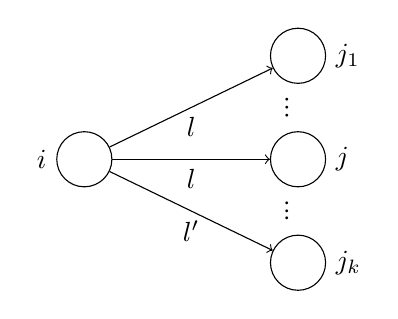
\begin{tikzpicture}
[
scale=1.0,
neuron-a/.style={circle,draw,minimum size = 07mm},
text-a/.style={black},
]
\node (n1) [neuron-a] at (0,0) {$ $};
\node (l1) [text-a,   left  = 00mm of n1]              {$i$};
\node (n2) [neuron-a, right = 20mm of n1]              {$ $};
\node (l2) [text-a,   right = 00mm of n2]              {$j$};
\node (d1) [text-a,   above = 03mm of n2, rotate =90]  {$...$};
\node (n3) [neuron-a, above = 06mm of n2]              {$ $};
\node (l3) [text-a,   right = 00mm of n3]              {$j_1$};
\node (d2) [text-a,   below = 03mm of n2, rotate =270] {$...$};
\node (n4) [neuron-a, below = 06mm of n2]              {$ $};
\node (l4) [text-a,   right = 00mm of n4]              {$j_k$};
\draw [->] (n1) -- (n2) node[midway, below] {$l$};
\draw [->] (n1) -- (n3) node[midway, below] {$l$};
\draw [->] (n1) -- (n4) node[midway, below] {$l'$};
\end{tikzpicture}                                                                                        
\end{center}                                                                                             
\caption{Neuron $i$ and Adjacent Neurons $j_1,...j_k$}\label{fig-snp2}
\end{figure} 

%===================================================================================================

\subsection{Spiking Rules with Delays}

An $n$-degree SNP system whose spiking rules have no delay ($d =0$) can be represented by a network 
of cell from the family $NC(n,\{a\}, REG^{\circ}, min)$. This section shows that $n$-degree SNP 
systems that use spiking rules with delay ($d > 0$) can simulated by network of cells from the 
family $NC(n, V, REG^{\circ}, min)$ where $V = \{a\} \cup \{x,r_1,...,r_f\}$. With the help of the
additional symbols from $\{x,r_1,...,r_f\}$, the behavior of a spiking rule with delay can be 
simulated by a set of interaction rules. 

Given a spiking rule $E/a^c \ra a^p;d$, the following behavior should be simulated:
\begin{itemize}
\item \emph{Delayed Spiking}: When the rule is applied at time $t$, the neuron should only send
      spikes to adjacent neurons at time $t+d$.
\item \emph{Prevention of Rule Application}: When a rule is active in a neuron, no other rules in 
      the neuron should be applied. 
\item \emph{Closing of Neuron}: When a neuron is closed, it should not receive spikes from other 
      neurons.
\end{itemize}

If a spiking rule with delay $d$ is applied at time $t$, it will be active for $d+1$ steps, from 
time $t$ to time $t+d$. The spiking rule is active $d+1$ steps but the neuron that applied the rule 
is only closed for $d$ steps, from time $t$ to time $t+d-1$. At time $t+d$, the neuron opens and it
sends out spikes to adjacent neurons. Time $t+d$ is the only time when the rule is still active 
but the neuron is already open. The scenario at time $t+d$ is the reason why the \emph{closing of
neuron} behavior is differentiated from the \emph{prevention of rule application} behavior.

Additional symbols will be used in order to simulate the behavior of spiking rules. The \emph{delay}
symbol $x$ is used to represent delay and the closed state of a neuron. If there are $x$ symbols 
in a  neuron, then that neuron is closed. The \emph{rule} symbols $r_1,...,r_f$ are used to 
represent rules being active in a neuron. If symbol $r_i \in \{r_1,...,r_f\}$ is in a neuron, then 
the spiking rule represented by $r_i$ is active in that neuron. If neuron $i$ contains the 
most number of spiking rules (with delay), then $f$ is the number of spiking rules (with delay) in
neuron $i$. For example, if neuron $A$ contains the most number of spiking rules, having 10 spiking
rules with delay, then $f=10$ and set of rule symbols that will be used is $\{r_1,...,r_{10}\}$.
Neuron $A$ will use symbols $r_1,...,r_{10}$ but another neuron in the same system, say neuron $B$, 
that only has two spiking rules with delay, will only use symbols $r_1$ and $r_2$. The alphabet of 
the network of cell will be $V = \{a,x,r_1,...,r_f\}$.

Let the spiking rule $R$ be in neuron $i$ and neurons $j_1,...,j_k$ are adjacent to neuron $i$ (see
Figure \ref{fig-snp}). The behavior of a spiking rule $R: E/a^c \ra a^p;d$ will be simulated by 
interaction rules with the following forms:

\begin{multicols}{2}
\begin{itemize}
\item $R_1:\ts [L^{\circ}(E_1)]_i / [a^c]_i \ra [x^{d-1}r]_i$ 
\item $R_2:\ts [L^{\circ}(E_2)]_i / [x]_i \ra \emptyset_n$
\item $R_3:\ts [L^{\circ}(E_3)]_i / [r]_i  \ra [a^p]_{j_1}\cdots[a^p]_{j_k}$ 
\item $E_1 = E$
\item $E_2 = a^*|x^+|r_1^*|\cdots|r_f^*$
\item $E_3 = a^*|r$
\end{itemize}
\end{multicols}

Interaction rule $R_1$ can only be applied if the neuron $i$ contains the multiset $a^n$ such that 
$a^n \in L^{\circ}(E_1)$ where $E_1=E$. This is almost the exact scenario when spiking rule $R$ can
be applied. i.e. $a^n \in L(E)$. The difference is that the regular expression $E_1$ of interaction
rule $R_1$ is over the alphabet $V=\{a,x,r_1,...,r_f\}$ and has a specific form specified in Section 
\ref{sec-preliminaries} while the regular expression $E$ of spiking rule $R$ is over the alphabet 
$O=\{a\}$. The regular expression $E_1$ specifies which spike counts can make interaction rule $R_1$ 
eligible but it also specifies that there should not be any delay symbol $x$ nor rule symbols 
$r_1,...,r_f$  for interaction rule to be eligible. For example, if an interaction rule uses the
regular expression $(a^2)^+$ and control language $L^{\circ}((a^2)^+) = \{a^2,a^4,a^6,...\}$, then
the rule is only eligible if there is an even number of spikes and there are no $x,r_1,...,r_p$ 
symbols in cell/neuron $i$. It is not sufficient to check only the number of spikes. The lack of 
delay and rule symbols means that the neuron/cell is open and there are no active rules. When 
interaction rule $R_1$ is applied at time $t$, it will consume the multiset $a^c$ in neuron $i$ and 
it will produce multiset $x^{d-1}r$ in the same neuron at time $t$. Symbol $r \in \{r_1,...,r_f\}$ 
is the rule symbol associated with spiking rule $R$ so it is one of the symbols produced by 
interaction rule $R_1$. The presence of delay symbols $x$ means neuron $i$ is now closed while the
presence of rule symbol $r$ means there is an active rule in neuron $i$.

Interaction rule $R_2$ simulates the delay countdown. Rule $R_2$ has a single eligibility condition,
the presence of at least one delay symbol $x$ in neuron $i$. It does not care about the spike count
nor the presence or absence of rule symbols $r_1,...,r_f$. This single condition is specified by the 
rule's regular expression $E_2 = a^*|x^+|r_1^*|\cdots|r_f^*$. When applied, interaction rule $R_2$ 
consumes a single delay symbol $x$ from neuron $i$ but does not produce any new symbols.

If interaction rule $R_1$ is applied at time $t$ and neuron $i$ has the multiset $a^n$, after rule
application neuron $i$ will now have the multiset $a^{n-c}x^{d-1}r$. From time $t+1$ to $t+d-1$, 
there will be at least one delay symbol $x$ in neuron $i$ which means interaction rule $R_2$ will be 
used in that time period. At time $t+d$, the multiset in neuron $i$ is $a^{n-c}r$. There are no more 
delay symbols $x$. There are only spike symbols and the single rule symbol $r$. Interaction rule 
$R_3$ that is associated with spiking rule $R$ is applied at time $t+d$. Regular expression
$E_3=a^*|r$ specifies that rule $R_3$ is eligible if the rule symbol $r$ is in neuron $i$ and there
are no other rule symbols nor delay symbols in the neuron. It does not care about the spike count.
When rule $R_3$ is applied at time $t$, rule symbol $r$ is consumed from neuron $i$ and $p$ spikes
are produced in each neuron $j \in \{j_1,...,j_k\}$ adjacent to neuron $i$.

Figure \ref{fig-delay-tab} shows the rules used by neuron $i$ in time $t$ to $t+d$ and the multiset 
in the neuron before and after the rule is applied.

\begin{figure}[H]
\begin{center}
\begin{tabular}{|l|l|c|l|}
\hline
\thead{Time}     & \thead{Multiset \\ (Before Rule Application)} & \thead{Rule} &\thead{Multiset\\(After Rule Application)}    \\ \hline
$t+0$    & $a^n$             & $R_1$ & $a^{n-c}x^{d-1}r$   \\ \hline
$t+1$    & $a^{n-c}x^{d-1}r$ & $R_2$ & $a^{n-c}x^{d-1}r$   \\ \hline
$...$    & $...$             & $R_2$ & $...$              \\ \hline
$t+d-2$  & $a^{n-c}x^{2}r$   & $R_2$ & $a^{n-c}x^{1}r$    \\ \hline
$t+d-1$  & $a^{n-c}xr$       & $R_2$ & $a^{n-c}r$         \\ \hline
$t+d$    & $a^{n-c}r$        & $R_3$ & $a^{n-c}$          \\ \hline
\end{tabular}
\end{center}
\caption{Multiset in Neuron $i$  Before and After an Interaction Rule is Applied (From Time $t$ to 
$t+d$)}
\label{fig-delay-tab}
\end{figure}

For each spiking rule $R$, there are corresponding interaction rules $R_1$ and $R_3$. For example, 
if there are two spiking rules with delay in a neuron, rules $R_u$ and $R_v$, then spiking rule 
$R_u$ will have the corresponding interaction rule $R_{u,1}$ that has the form of interaction rule 
$R_1$ and interaction rule $R_{u,3}$ that has the form of interaction rule $R_3$ while spiking rule $R_v$
will have interaction rules $R_{v,1}$ and $R_{v,3}$. The neuron will only have a single interaction
rule $R_2$ since this rule is not specific to a single spiking rule. To simulate the behavior of
the spiking rule $R_u$, interaction rules $R_{u,1}$, $R_2$, and $R_{u,3}$ are used and to simulate
the behavior of spiking rule $R_v$, interaction rules $R_{v,1}$, $R_2$, and $R_{v,3}$ are used.
The delay of the spiking rule is encoded in interaction rule $R_1$ while the action (number of
spikes produces) is encoded in interaction rule $R_3$. Interaction rule $R_2$ is used to implement
the delay countdown mechanism used by all spiking rules with delay.

The \emph{prevention of rule application} behavior is implemented using interaction rule $R_1$ (is 
not eligible if there are rule symbols in the neuron) while the \emph{spiking delay} behavior is 
implemented using all three interaction rules $R_1$ (produces delay objects), $R_2$ (countdown
mechanism), $R_3$ (actual spike production). Interaction rule $R_1$ produces delay symbols in the 
neuron that indicate that the neuron is closed but there are no mechanisms preventing other neurons
from sending spikes. For example, if there is a synapse from neuron $h$ to neuron $i$, $R_3$ 
interaction rules in neuron $h$ should be modified such that they will not produce spikes in neuron
$i$ if neuron $i$ is closed. Let $R_3:\ts [L^{\circ}(E_3)]_h / [r]_h  \ra \cdots[a^p]_{i}\cdots$ be
an interaction rule in neuron $h$. The rule produces the multiset $a^p$ in neuron $i$ as specified
by ${[a^p]}_{i}$ on the right of the arrow. Interaction rule $R_3$ has to be modified in such a
way as to not send the multiset $a^p$ to neuron $i$ if neuron $i$ is closed or is about to close.
Neuron $i$ is closed if there is at least one delay symbol $x$ in the neuron and neuron $i$ is about 
to close if there are no delay symbols in the neuron but there is at least one rule with delay in 
neuron $i$ that is eligible. Interaction rule $R_3$ will have to check the multiset in neuron $i$
to see if there are any delay symbols in the neuron or to see if the multiset in neuron $i$ makes
rules with delay in neuron $i$ eligible. For simplicity, we will call a neuron \emph{closed} if it 
is actually closed (neuron with delay symbols) or if it is about to close (with eligible rules with
delay). Interaction rule $R_3$ will be modified to include a control language that is associated 
with neuron $i$. i.e. Interaction rule $R_3$ will have the form 
${[L^{\circ}(E_3)]}_h{[L^{\circ}(E_i)]}_i/{[r]}_h\ra \cdots {[a^p]}_i \cdots$. The control language
$L^{\circ}(E_i)$ contains all multisets that signify that neuron $i$ is open. The regular expression
$E_i$ specifies multisets that do not contain delay symbol $x$ and do not contains spike counts that
will make a rule with delay in neuron $i$ to be eligible. 

We look at an SNP subsystem in Figure \ref{fig-snp3} for a specific example. For now, our concern is
translating the spiking rule $r_u: a^7/a^7 \ra a^3: 6$ in neuron $h$ to a set of interaction rules. 
At most, there are two rules with delay in a neuron so the alphabet for the corresponding network of
cells is $V=\{a,x,r_1,r_2\}$. We will use the rule symbol $r_1$ for spiking rule $r_u$ in neuron 
$h$. 

\begin{figure}[H]
\begin{center}                                                                                           
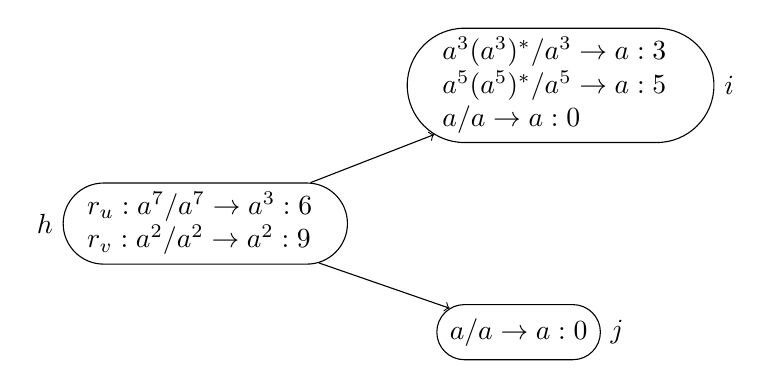
\begin{tikzpicture}
[
scale=1.0,
neuron-a/.style={rounded rectangle,draw,minimum size = 07mm},
text-a/.style={black},
]
\node (nh) [neuron-a, text width = 30mm] at (0,0)       {$r_u: a^7/a^7 \ra  a^3: 6$ \\
                                                         $r_v: a^2/a^2 \ra a^2:  9$};
\node (l1) [text-a,   left  = 00mm of nh]               {$h$};
\node (ni) [neuron-a, above right= 05mm and 20mm of nh,text width=30mm] {$a^3(a^3)^*/a^3 \ra a:3$ \\  
                                                                         $a^5(a^5)^*/a^5 \ra a:5$ \\
                                                                         $a/a \ra a:0$};
\node (li) [text-a,   right  = 00mm of ni]              {$i$};
\node (nj) [neuron-a, below right= 05mm and 20mm of nh] {$a/a \ra a:0$};
\node (lj) [text-a,   right  = 00mm of nj]              {$j$};
\draw [->] (nh) -- (ni) node[midway] {$ $};
\draw [->] (nh) -- (nj) node[midway, below] {$ $};
\end{tikzpicture}                                                                                        
\end{center}                                                                                             
\caption{Example SNP System}\label{fig-snp3}
\end{figure} 

Initially, spiking rule $r_u: a^7/a^7 \ra a^3:6$ will have the corresponding interaction rules:

\begin{itemize}
\item $R_{u,1}:\ts [L^{\circ}(a^7)]_h / [a^7]_h \ra [x^{5}r_1]_h$ 
\item $R_{u,2}:\ts [L^{\circ}(a^*|x^+|r_1^*|r_2^*)]_h / [x]_h \ra \emptyset_n$
\item $R_{u,3}:\ts [L^{\circ}(a^*|r_1)]_h / [r_1]_h \ra [a^3]_{i}[a^3]_{j}$
\end{itemize}

Interaction rule $R_{u,1}$ only activates if there is exactly $7$ spikes in neuron $h$ and there
are no delay or rule symbols. When applied, say at time $t$, interaction rule $R_{u,1}$, consumes 
$7$ spikes and produces the multiset $x^5r_1$ in neuron $h$. Multiset $x^5$ represents $5$ 
additional time steps (time $t+1$ to $t+5$) when neuron $h$ is closed (excluding the current time 
step $t$). The rule symbol $r_1$ represents spiking rule $r_u$ being active. Interaction rule 
$R_{u,2}$  will be applied as long as there are still delay symbols in neuron $h$. Interaction rule 
$R_{u,2}$ only consumes a single delay symbol $x$ per step and it will be used for 5 steps (at time 
$t+1$ to $t+5$). In total, neuron $h$ is closed for 6 steps at time $t$ to $t+5$. At time $t+6$, 
there will be no more delay symbols but the rule symbol $r_1$ is still in neuron $h$ which means 
interaction rule $R_{u,3}$ will be applied consuming rule symbol $r_1$ in neuron $h$ and producing 
the multiset $a^3$ in both neuron $i$ and neuron $j$.

Interaction rule $R_{u,3} $always produces spikes in neuron $j$. This should not be the case for
neuron $i$.Neuron $i$ contains spiking rules with delay which means interaction rule $R_{u,3}$ 
should check if neuron $i$ is closed or open and only produce spikes in neuron $i$ if neuron $i$ is
open. Two versions of interaction rule $R_{u,3}$ should be in neuron $h$, a version that checks if 
neuron $i$ is open and sends spikes to both neuron $i$ and neuron $j$ (we denote this rule as 
$R_{u,3}$) and a version that checks if neuron $i$ is closed and sends spikes only to neuron $j$ 
(we denote this rule as $\overline{R}_{u,3}$). Interaction rules $R_{u,3}$ and $\overline{R}_{u,3}$ 
are the following:

\begin{itemize}
\item $R_{u,3}:\ts {[L^{\circ}(a^*|r_1)]}_h {[L^{\circ}(E_i)]}_i / {[r_1]}_h \ra {[a^3]}_{i}{[a^3]}_{j}$
\item $\overline{R}_{u,3}:\ts {[L^{\circ}(a^*|r_1)]}_h {[L^{\circ}(E'_i)]}_i/ {[r_1]}_h \ra {[a^3]}_{j}$
\item where $E'_i =  a^*| x^+ | r_1^* | r_2^* \cup a^3(a^3)^* \cup a^5(a^5)^*$
\end{itemize}

Interaction rule $\overline{R}_{u,3}$ uses the control language $L^{\circ}(E'_i)$. The regular 
expression $E'_i$ specifies the set of multisets that signify that neuron $i$ is closed. Regular 
expression $E'_i$ is composed of three sub-expressions connected by the union operator $\cup$. The
sub-expression $a^*|x^+|r_1^*|r_2^*$ represents the multisets that contain at least one delay symbol
$x$ which means neuron $i$ is closed. The sub-expressions $a^3(a^3)^*$ and $a^5(a^5)^*$ are the 
regular expressions of spiking rules with delay in neuron $i$. If neuron $i$ contains a multiset
that is specified by either $a^3(a^3)^*$ or $a^5(a^5)^*$, then neuron $i$ is about to close. By
combining the three sub-expressions using the union operator, the resulting expression $E'_i$ 
specifies all multisets that make neuron $i$ a closed neuron. When activated, interaction rule 
$\overline{R}_{u,3}$ only produces the multiset $a^3$ in neuron $j$.

Interaction rule $R_{u,3}$ uses the complementary control language $L^{\circ}(E_i)$. If regular
expression $E'_i$ specifies multisets where neuron $i$ is closed, regular expression $E_i$ specifies
multisets where neuron $i$ is open. When activated, interaction rule $R_{u,3}$ produces the multiset
$a^3$ in both neuron $i$ and neuron $j$.

In general, if neuron $h$ is connected to $q$ neurons with spiking rules with delay, then for a 
spiking rule $r_{u}$ in neuron $h$ the corresponding set of interaction rules contains the rules
$R_{u,1}$, $R_{u,2}$ and $2^q$ versions of $R_{u,3}$. For example, if neuron $h$ is connected to two
neurons ($q=2$) both with spiking rules with delay, say neuron $a$ and neuron $b$, then the spiking
rule $r_u$ will have $2^q = 2^2 = 4$ versions of interaction rule $R_{u,3}$, one for each of the 
following cases:

\begin{itemize}
\item $R_{u,3}$ for the case when both neuron $a$ and neuron $b$ are closed.
\item $R_{u,3}$ for the case when neuron $a$ is closed and neuron $b$ is open.
\item $R_{u,3}$ for the case when neuron $a$ is open and neuron $b$ is closed.
\item $R_{u,3}$ for the case when both neuron $a$ and neuron $b$ are open.
\end{itemize}

In summary, in order to simulate the behavior (delay spiking, prevention of rule application,
closing of neuron) a spiking rule $r_u$, additional symbols and three types of interaction rules 
should be created, interaction rules $R_1$, $R_2$, $R_3$. For spiking rule $r_u$, the $R_1$ 
interaction rule is denoted by $R_{u,1}$, the $R_2$ interaction rule is denoted by $R_{u,2}$, and
the $R_3$ interaction rule is denoted by $R_{u,3}$. Interaction rule $R_{u,1}$ contains the 
information about spiking rule $r_u$'s regular expression, delay and the number of spikes it 
consumes. Interaction rule $R_{u,3}$ contains the information about spiking rule $r_u$'s action
(the number of spikes it produces and the target neurons). Interaction rule $R_{u,2}$ is used for
the delay countdown mechanism and does not contain information particular to spiking rule $r_u$ 
which means it can be reused by other spiking rules with delay in the same neuron. i.e. If a neuron
has two spiking rules with delay, $r_u$ and $r_v$, their corresponding $R_2$ interaction rules
$R_{u,2}$ and $R_{v,2}$ is the same interaction rule. If the target neurons in $R_{u,3}$ can close,
then multiple versions of $R_{u,3}$ should be created for the different scenarios where some of the
targets neurons are closed while some target neurons are open.

%===================================================================================================

\subsection{}


%===================================================================================================


\section{Discussion}



%===================================================================================================

\appendix{}

\section*{Appendices}\label{app}
\section{Derivation Modes}\label{app-derivation}

\cite{freund-2007-ff-1}

\begin{itemize}                                                                                       
   \item $Applicable(\Pi, C, \delta) \subseteq Applicable(\Pi, C)$ - Set of applicable multisets of 
         rules in $\delta$-mode.                                                                                 
   \item $Applicable(\Pi, C, asyn) = Applicable(\Pi, C)$ - \textit{Asynchronous} Mode ($\delta = 
         asyn$).            
   \item $Applicable(\Pi, C, sequ) = \{R' \in Applicable(\Pi, C) \ts | \ts |R'|=1\}$ - 
         \textit{Sequential} Mode ($\delta = sequ$) - One rule instance only.                                                         
   \item $Applicable(\Pi, C, max) = \{R' \in Applicable(\Pi, C) \ts | \not\exists R'' \in Applicable(\Pi, C), \ts R' i   
         \not\subseteq R'' \}$ - \textit{Maximally Parallel} Mode ($\delta = max$) - Adding any rule 
         to a maximally parallel $R'$ will result in an inapplicable multiset of rules.                 
   \item $Applicable(\Pi, C, min) = \{R' \in Applicable(\Pi, C) \ts | \ts \not\exists R'' \in Applicable(\Pi,C), \ts R'   
         \subseteq R'', \exists j, (R''-R') \cap R_j \neq \emptyset, R' \cap R_j = \emptyset\}$                                                                                              
         - \textit{Minimally Parallel} Mode ($\delta = min$) - There is no partition                    
          $R = R_1 \cup R_2 \cup \cdots \cup R_h$. Rule set $R$ is be partitioned.                      
          $R' \subseteq R''$. $R''$ `extends' R'.                                                       
   \item $\delta \in \{asyn, sequ, max, min\}$ - Basic derivation modes                                 
   \item $Applicable(\Pi, C, max_{rule}\delta) = \{R' \in Applicable(\Pi, C, \delta) \ts | \ts \not\exists R''        
         \in Applicable(\Pi,C, \delta) \ts |R''| > |R'|\}$\\ - \textit{Maximum Rules} $\delta$-Mode.           
   \item $Applicable(\Pi, C, max_{set}\delta) = \{R' \in Applicable(\Pi, C, \delta) \ts | \ts \not\exists R'' \in  
         Applicable(\Pi,C, \delta) \ts ||R''|| > ||R'||\}$\\ - \textit{Maximum Sets (Partitions)} $            
         \delta$-Mode.                                                                                  
   \item $Applicable(\Pi, C, all_{set}\delta) = \{R' \in Applicable(\Pi, C, \delta) \ts | \ts \forall j, 1 \leq j  
         \leq h, (R_j \cap \bigcup_{X \in Applicable(\Pi,C)} X \neq \emptyset) \rightarrow (R_j \cap R'    
         \neq \emptyset)\}$ - \textit{All Set} $\delta$-Mode.                                           
\end{itemize}

%===================================================================================================

\section{Halting Conditions}\label{app-halt}

\begin{enumerate}
\item Total Halting
\item Adult Halting
\item Partial Halting 
\end{enumerate}

%===================================================================================================
\bibliographystyle{plain}
\bibliography{cs-290}

\end{document}

%==================================================================================================



